\documentclass[
  % Schriftgröße
  11pt,
  % Ein- oder Zweiseitiges Dokument (oneside, twoside)
  oneside,
  a4paper,
  % Kein Punkt am Ende der Nummerierung
  numbers=noenddot,
  % Literaturverzeichnis ins ToC
  bibliography=totoc,
  % Abbildungs- und Tabellenverzeichnis ins ToC
  listof=totoc,
  % Linie unter Kopfzeile
  headsepline,
  % Absatz nicht einrücken
  %parskip,
  % Kein vertikaler Abstand in Verzeichnissen zwischen unterschiedlichen Kapitel
  %listof=nochaptergap
]{scrreprt}

\usepackage{etex}
\usepackage[utf8]{inputenc}
\usepackage{lmodern}
% wichtig für Trennung von Wörtern mit Umlauten
\usepackage[T1]{fontenc}
\usepackage{lmodern}

% verbesserter Randausgleich
\usepackage{microtype}

\usepackage{url}
% URLs in Normaler Schrift
%\urlstyle{rm}

\usepackage{multirow}
\usepackage[colorlinks=true,linkcolor=black,citecolor=black,urlcolor=black,bookmarksdepth=5]{hyperref}
% deutsche Trennregeln
\usepackage[ngerman]{babel}

% Länge der Fußnote
\interfootnotelinepenalty=10000

\usepackage{paralist}

% Abbildungen
\usepackage{graphicx}
\usepackage{pdfpages}
\usepackage{dirtree}

% Mathematische Formeln
\usepackage{amsmath}
\usepackage{amssymb}
\usepackage{amstext}
\usepackage{amsfonts}
\usepackage{mathrsfs}
\usepackage{array}
\usepackage{mathtools}
\usepackage{wasysym}
\usepackage[a]{esvect}

%  SI units
\usepackage[
  binary-units=true,
  output-decimal-marker={,},
]{siunitx}

\usepackage[square]{natbib}
\setlength{\bibsep}{0.25cm}
\renewcommand{\bibfont}{\small}
\renewcommand*{\bibpreamble}{\interlinepenalty10000\relax}

% Setze Autoren in Kapitälchen
\makeatletter
  \renewcommand*{\NAT@nmfmt}[1]{\textsc{#1}}
\makeatother

\usepackage{textcomp}

% Erlaube Underscores in Fließtext ohne Escape
\usepackage[strings]{underscore}

\usepackage{xspace}

% Gänsefüßchen unten
\newcommand{\gu}{\glqq{}}
% Gänsefüßchen oben
\newcommand{\go}{\grqq\xspace}

% sharp symbol (#)
\newcommand{\textsharp}{\texttt{\#}}

% Spezielles eingekringeltes Plus
\newcommand{\plus}{\text{{\large\textcircled{\normalsize \texttt{+}}}}}

% hochgestelltes Copyright-Symbol
\def\CopTop{\textsuperscript{\textcopyright}}

\usepackage{pifont}
\newcommand{\cmark}{\ding{51}}
\newcommand{\xmark}{\ding{55}}
\newcommand{\quadrat}{\ding{110}}
\newcommand{\kreis}{\ding{108}}

\usepackage[automark]{scrpage2}
\automark[section]{chapter}
\pagestyle{scrheadings}
\clearscrheadfoot
\ihead{\leftmark}
\ohead{\pagemark}
\renewcommand*{\chapterpagestyle}{scrheadings}
\renewcommand*{\indexpagestyle}{scrheadings}
\usepackage[left=30mm,right=38mm,top=30mm,bottom=20mm]{geometry}

\RedeclareSectionCommand[
  beforeskip=-1\baselineskip,
  afterskip=0.4\baselineskip
]{chapter}

% Kapitelpräfixgröße
\setkomafont{chapterprefix}{\large}
% Kapitelgröße
\setkomafont{chapter}{\LARGE}
% Paragraphen/Absatzabstand
\setlength{\parskip}{0.7EM}

% Fußnoten eingerückt untereinander
\deffootnote[]{1em}{1em}{\textsuperscript{\thefootnotemark\ }}

% Fußnoten über alle Kapitel absolut
\usepackage{remreset}
\makeatletter
\@removefromreset{footnote}{chapter}
\makeatother

\newcommand{\sffett}[1]{\textsf{\textbf{#1}}}
\newcommand{\mathsfbold}[1]{\boldsymbol{\mathsf{#1}}}

% 1,5-zeiligen Zeilenabstand
\usepackage{setspace}
\onehalfspacing

\usepackage{float}

\usepackage{chngcntr}

% Anhang
\renewcommand\appendix{\par
  % Inhaltsverzeichnis ohne Anhangbilder, aber im Anhang nummeriert
  \captionsetup{list=false}
  \counterwithin*{figure}{section}
  \counterwithin*{table}{section}
  \counterwithin*{algorithm}{section}
  \counterwithin*{lstlisting}{section}
  \renewcommand\thesection{\Alph{section}}
  \renewcommand\thefigure{Abb.~\Alph{section}.\arabic{figure}}
  \renewcommand\thetable{Tab.~\Alph{section}.\arabic{table}}
  \renewcommand{\thelstlisting}{\thesection.\arabic{lstlisting}}
  \renewcommand{\thealgorithm}{\thesection.\arabic{algorithm}}
}

\usepackage{xcolor}

\definecolor{lightgray}{RGB}{240 240 240}

% Farbakzente der Office 2016 Standardvorlage
\definecolor{akzent1}{RGB}{219 0 49}
\definecolor{akzent2}{RGB}{100 18 27}
\definecolor{akzent3}{RGB}{159 19 37}
\definecolor{akzent4}{RGB}{233 78 27}
\definecolor{akzent5}{RGB}{243 146 0}
\definecolor{akzent6}{RGB}{249 178 51}

% Inhaltsverzeichnis
\setcounter{secnumdepth}{2}
\renewcommand*{\theparagraph}{\thesubsubsection.\alph{paragraph}}
\setcounter{tocdepth}{2}
\usepackage{tocstyle}
\usetocstyle{allwithdot}

% Anhang richtig verlinkt im Inhaltsverzeichnis
\renewcommand*{\theHsection}{\thesection}


% Tabellen- und Abbildungsverzeichnis
% Einrücken verhindern
% Default: 1.5em/2.3em
\makeatletter
  \renewcommand*\l@figure{\@dottedtocline{1}{0em}{2.3em}}
  \let\l@table\l@figure
\makeatother

\renewcommand{\thefigure}{Abb.~\arabic{chapter}.\arabic{figure}}
\renewcommand{\thetable}{Tabelle~\arabic{chapter}.\arabic{table}}
\renewcommand{\theequation}{Gl.~\arabic{chapter}.\arabic{equation}}
\renewcommand*{\figureformat}{\thefigure}
\renewcommand*{\tableformat}{\thetable}
\renewcommand*{\captionformat}{: }

% Bild-/Tabellenunterschriften klein & serifenlos
\addtokomafont{caption}{\small\sffamily}
% Bild-/Tabelllabel fett & serifenlos
\addtokomafont{captionlabel}{\sffamily\bfseries}

% Doppelpunkt nach Nummern
\AtBeginDocument{
  \addtocontents{lof}{\protect\def\protect\autodot{:}}
  \addtocontents{lot}{\protect\def\protect\autodot{:}}
}

\usepackage{caption}

% Abkürzungsverzeichnis
\usepackage[
  % fügt das Verzeichnis dem Inhaltsverzeichnis zu
	toc,
  % Abkürzungsverzeichnis hinzufügen
  acronym,
  % keine Seitenzahlen
  nonumberlist,
  % kein Punkt am Ende der Beschreibung
  nopostdot,
  % Kein Abstand zwischen Alphabetgruppen
  nogroupskip
]{glossaries}

\newglossary[slg]{symbols}{sls}{slo}{Symbolverzeichnis}

% Benutzerdefinierte Acronymeigenschaften
% user1
\let\acrlonggen\glsuseri
% user2
\let\acrlongpldat\glsuserii

% Style auf long aufbauend aber mit verbessertem Abstand
\newglossarystyle{longspace}{%
  \setglossarystyle{long}
  \renewenvironment{theglossary}%
     {\begin{longtable}[l]{@{}p{0.15\textwidth}@{}p{0.85\textwidth}}}
     {\end{longtable}}
  \renewcommand{\glossentry}[2]{%
    \glsentryitem{##1}\glstarget{##1}{\glossentryname{##1}} &
    \glossentrydesc{##1}\glspostdescription\space ##2\tabularnewline[5mm]
  }%
  \renewcommand{\subglossentry}[3]{%
     &
     \glssubentryitem{##2}%
     \glstarget{##2}{\strut}\glossentrydesc{##2}\glspostdescription\space
     ##3\tabularnewline[2mm]
  }%
}

% Generiere später die Glossary Dateien
\makeglossaries

\usepackage{tabularx}
\usepackage{varwidth}
% Ermöglicht Tabellen über Seitenumbruch
\usepackage{longtable}
% Fußnoten in Tabellen
\usepackage[]{threeparttable}
\usepackage{booktabs}
\usepackage{pdflscape}
\usepackage{colortbl}
% Liste in Tabelle
\usepackage{enumitem}
% Gestrichelte Linien in Tabellen
\usepackage{arydshln}
\usepackage{hhline}
% Rotation einr Tabelle
\usepackage{rotating}

% Kurzbefehl für rotatebox um 90°
\newcommand{\rot}[1]{\rotatebox{90}{#1~}}

% Kurzer Befehl für multicolumn
\newcommand{\mc}[3]{\multicolumn{#1}{#2}{#3}}

% Anpassung der Zellhöhe
\makeatletter
  \renewenvironment{table}{
  	\renewcommand{\arraystretch}{1.3}
  	\@float{table}
  }{\end@float}
\makeatother

% Fußzeile über gesamte Breite, kann in jeder table-Umgebung seperat gesetzt werde
%\renewcommand{\TPTminimum}{\linewidth}

\usepackage{algorithm}
\usepackage{algpseudocode}

\renewcommand{\thealgorithm}{\thechapter.\arabic{algorithm}}

\renewcommand{\listalgorithmname}{Algorithmusverzeichnis}
\floatname{algorithm}{Algorithmus}

% Entferne Einrückung bei Algorithmusverzeichnis
\patchcmd{\listof}{1.5em}{0pt}{}{}

% Übersetzung der Schlüsselwörter
\renewcommand{\algorithmicrequire}{\textbf{Eingabe:}}
\renewcommand{\algorithmicensure}{\textbf{Ausgabe:}}
\renewcommand{\algorithmicend}{\textbf{end}}
\renewcommand{\algorithmicif}{\textbf{if}}
\renewcommand{\algorithmicthen}{\textbf{then}}
\renewcommand{\algorithmicelse}{\textbf{else}}
\newcommand{\algorithmicelsif}{\algorithmicelse\ \algorithmicif}
\newcommand{\algorithmicendif}{\algorithmicend\ \algorithmicif}
\renewcommand{\algorithmicfor}{\textbf{for}}
\renewcommand{\algorithmicforall}{\textbf{for all}}
\renewcommand{\algorithmicdo}{\textbf{do}}
\newcommand{\algorithmicendfor}{\algorithmicend\ \algorithmicfor}
\renewcommand{\algorithmicwhile}{\textbf{while}}
\newcommand{\algorithmicendwhile}{\algorithmicend\ \algorithmicwhile}
\renewcommand{\algorithmicloop}{\textbf{loop}}
\newcommand{\algorithmicendloop}{\algorithmicend\ \algorithmicloop}
\renewcommand{\algorithmicrepeat}{\textbf{repeat}}
\renewcommand{\algorithmicuntil}{\textbf{until}}
\newcommand{\algorithmicprint}{\textbf{print}}
\renewcommand{\algorithmicreturn}{\textbf{return}}
\newcommand{\algorithmictrue}{\textbf{true}}
\newcommand{\algorithmicfalse}{\textbf{false}}

\usepackage{listings}

\usepackage{caption}
\newenvironment{code}{\captionsetup{type=lstlisting}\vspace{4mm}}{\vspace{2mm}}
\captionsetup[lstlisting]{skip=1mm}


\makeatletter
\AtBeginDocument{%
\renewcommand\lstlistoflistings{\bgroup
  \let\contentsname\lstlistlistingname
  \def\l@lstlisting##1##2{\@dottedtocline{1}{0pt}{0pt}{Listing ##1}{##2}}
  \let\lst@temp\@starttoc \def\@starttoc##1{\lst@temp{lol}}%
  \tableofcontents \egroup}
}
\makeatother

\def\lstlistlistingname{Quellcodeverzeichnis}

\lstset{
  nolol=true,
  numbers=left,
  xleftmargin=0.8mm,
  framexleftmargin=0.8mm,
  numberstyle=\tiny\color{black},
  numberblanklines=true,
  language=Python,
  basicstyle=\footnotesize\ttfamily,
  frame=tb,
  escapeinside=||,
  keepspaces=true,
  breaklines=true,
  breakindent=0mm,
  postbreak=\raisebox{0ex}[0ex][0ex]{\color{gray}\ensuremath{\hookrightarrow\space\space}},
  columns=flexible,
  showstringspaces=false,
  commentstyle=\color{gray},
  upquote=true,
  literate=
  {ä}{{\"a}}1 {ë}{{\"e}}1 {ï}{{\"i}}1 {ö}{{\"o}}1 {ü}{{\"u}}1
  {Ä}{{\"A}}1 {Ë}{{\"E}}1 {Ï}{{\"I}}1 {Ö}{{\"O}}1 {Ü}{{\"U}}1
  {ß}{{\ss}}1
  {€}{{\EUR}}1 {°}{\SI{}{\degree}}1
}


\usepackage{calc}

\newlength{\codelettersize}
\settowidth{\codelettersize}{\ttfamily\footnotesize{i}}

\makeatletter
  \newcommand{\nextline}[3][0]{
    \\[3mm] \rule{0cm}{0cm} \hspace{-4.2\codelettersize}$\cdot\cdot$\hspace{2\codelettersize}\hspace{#1\codelettersize}\color{gray}\itshape #3 \\[3mm]
    \setcounter{lstnumber}{#2-1}
    \aftergroup\lst@numberfirstlinefalse
  }
\makeatother

% Save the original way of printing the number (Custom Line Numbering)
\let\othelstnumber=\thelstnumber
\def\createlinenumber#1#2{
  \edef\thelstnumber{%
    \unexpanded{%
      \ifnum#1=\value{lstnumber}\relax
      #2%
      \else}%
    \expandafter\unexpanded\expandafter{\thelstnumber\othelstnumber\fi}%
  }
  \ifx\othelstnumber=\relax\else
  \let\othelstnumber\relax
  \fi
}

% Änderung des Aufzählungszeichens 1. Ebene
\renewcommand{\labelitemi}{--}

% Erweitere Beschreibungsliste
\usepackage{expdlist}


\hypersetup{
  bookmarksnumbered,
  pdfauthor={Stephan Müller},
  pdftitle={Template für eine Bachelor- oder Masterthesis},
  pdfkeywords={Latex, Thesis, Bachelor, Master}
}

% Abkürzungen und Symbole laden
% Anleitung zu Glossaries und Acronyms:
% https://en.wikibooks.org/wiki/LaTeX/Glossary

\newacronym[
  plural={Bilder pro Sekunde},
  longplural={Bilder pro Sekunde},
  user2={Bildern pro Sekunde}
]{bps}{BpS}{Bild pro Sekunde}


\newglossaryentry{naiive}{
  name=na\"{\i}ve,
  description={is a French loanword (adjective, form of naïf) indicating having or showing a lack of experience, understanding or sophistication},
  sort=naiive
}

\newglossaryentry{Linux}{
  name=Linux,
  description={is a generic term referring to the family of Unix-like computer operating systems that use the Linux kernel},
  plural=Linuces
}

\longnewglossaryentry{computer}{name=computer}{
  is a programmable machine that receives input, stores and manipulates data, and provides output in a useful format
}
\newglossaryentry{real number}{
  name={real number},
  description={include both rational numbers, such as $42$ and $\frac{-23}{129}$, and irrational numbers, such as $\pi$ and the square root of two; or, a real number can be given by an infinite decimal representation, such as $2.4871773339\ldots$ where the digits continue in some way; or, the real numbers may be thought of as points on an infinitely long number line},
  symbol={\ensuremath{\mathbb{R}}}
}


\newglossaryentry{euro}{
  name={\texteuro},
  symbol={-},
  description={Währung der Europäischen Union},
  type=symbols,
  sort=euro
}

\newglossaryentry{dollar}{
  name={\textdollar},
  symbol={-},
  description={Währung der Vereinigten Staaten von Amerika},
  type=symbols,
  sort=dollar
}

\newglossaryentry{cent}{
  name={\textcent},
  symbol={-},
  description={Centbeträge von Währungen},
  type=symbols,
  sort=cent
}

\newglossaryentry{chf}{
  name={CHF},
  symbol={-},
  description={Währung der Schweiz},
  type=symbols,
  sort=chf
}

\newglossaryentry{gu}{
  name={\gu Text},
  symbol={-},
  description={Gänsefüßchen unten mit \texttt{\textbackslash gu Text}},
  type=symbols
}

\newglossaryentry{go}{
  name={Text\go},
  symbol={-},
  description={Gänsefüßchen oben mit \texttt{Text\textbackslash go}},
  type=symbols
}

\glsaddall

% Hinzufügen von Textplatzhaltern
\usepackage{blindtext}

\begin{document}

% Füge Tabellenverzeichnis in Inhaltsverzeichnis ein
\addtocontents{lot}{\vskip 0.4cm}
% Füge Abbildungsverzeichnis in Inhaltsverzeichnis ein
\addtocontents{lof}{\vskip 0.4cm}

\newgeometry{left=30mm,right=25mm,top=30mm,bottom=20mm}
\phantomsection\pdfbookmark{Deckblatt}{deckblatt}
\begin{titlepage}
  \begin{center}
    \huge{\mdseries\rmfamily
      Vorlage für Abschlussarbeiten der Fakultät für Wirtschaftswissenschaften an der Hochschule Karlsruhe}
    \vspace{0.5\baselineskip}\\
    \mdseries\rmfamily\normalsize
      Template for degree theses at Faculty of Management Science and Engineering at Karlsruhe University of Applied Sciences\\
    \vspace{2\baselineskip}
    \mdseries\rmfamily\normalsize
      Master-Thesis\\
    \mdseries\rmfamily\normalsize
      im Studiengang Wirtschaftsingenieurwesen\\
    \vspace{2\baselineskip}
    \mdseries\rmfamily\normalsize
      zur Erlangung des akademischen Grades\\
    \textsf{\textbf{Master of Science (M.Sc.)}}\\
    \vspace{3\baselineskip}
    \mdseries\rmfamily\normalsize
      vorgelegt von\\
    \textsf{\textbf{Vorname Nachname}}\\
    \mdseries\rmfamily\normalsize
      aus Karlsruhe\\
    \vspace{3\baselineskip}
  \end{center}
  \begin{flushleft}
    \begin{tabular}{lccl}
      Erstkorrektor:  & & & Prof. Dr. Rainer Zufall\\
      Zweitkorrektor: & & & Prof. Dr. Ernst Haft\\
      & & &\\
      Inhaltliche Mitbetreuung:
      & & & Anna Nass, M.Sc.\\
      & & & Klaus Uhr, M.Sc.\\
      & & &\\
      Matr.-Nr.: & & & 99999\\
      E-Mail: & & & vorname@nachname.de\\
      & & &\\
      Bearbeitungszeitraum:& & & 01.01.\the\year -- 31.12.\the\year\\
      Tag der Einreichung: & & & 31.12.\the\year \\
    \end{tabular}
    \vspace{3\baselineskip}\\
  \end{flushleft}
  \begin{center}
    \mdseries\rmfamily\normalsize Fakultät für Wirtschaftswissenschaften\\
    \mdseries\rmfamily\normalsize Hochschule Karlsruhe -- Technik und Wirtschaft\\
    \the\year
  \end{center}

\end{titlepage}


\newgeometry{left=30mm,right=38mm,top=30mm,bottom=20mm}

\chapter*{Kurzfassung}
\thispagestyle{empty}
\blindtext
\vspace{2\baselineskip}

\subsubsection*{Abstract}
\textit{\blindtext@english}
\vspace{10\baselineskip}


% Schlüsselwortliste
\paragraph*{Schlüsselwortliste:}
Wort 1, Wort 2, Wort 3

\vspace{-1\baselineskip}

\paragraph*{Keywords:}
\textit{Word 1, Word 2, Word 3}
\clearpage



\chapter*{Danksagung}
\thispagestyle{empty}
\blindtext


\pagenumbering{Roman}
\setcounter{page}{1}

% Erstelle Lesezeichen für das Inhaltsverzeichnis
\cleardoublepage\phantomsection\pdfbookmark{\contentsname}{toc}
% Inhaltsverzeichnis
\tableofcontents

% Tabellenverzeichnis
\setcounter{tocdepth}{2}
\listoftables

% Abbildungsverzeichnis
\listoffigures

% Algorithmusverzeichnis
\listofalgorithms

% Quelltextverzeichnis
%\renewcommand*{\thelstlisting}{List.~\arabic{lstlisting}}
%\renewcommand*{\lstlistlistingname}{Quelltextverzeichnis}
\lstlistoflistings

% Abkürzungsverzeichnis & Symbolverzeichnis
\printglossary[
  title=Glossar,
  toctitle=Glossar
]
\printglossary[
  title=Abkürzungsverzeichnis,
  toctitle=Abkürzungsverzeichnis,
  type=\acronymtype
]
\printglossary[
  title=Symbolverzeichnis,
  toctitle=Symbolverzeichnis,
  type=symbols,
  style=symbolstyle
]

% Inhalt der Arbeit
\pagenumbering{arabic}
\setcounter{page}{1}
\chapter{Einleitung}
\label{chap:einleitung}


\section{Motivation und Problemstellung}
\label{sec:motivation-und-problemstellung}
Viele Studenten würden gerne auf die Nachteile von Office Word beim Schreiben einer Abschlussarbeit verzichten. Die Alternative dazu ist \LaTeX, ein qualitativ hochwertiges Schriftsatzprogramm. Leider ist die Bedienung für Einsteiger nicht gerade intuitiv und die anfängliche Einarbeitung in die neue Umgebung sehr mühsam. Mit einer pofessionallen Vorlage, die nach dem Herunterladen ohne weitere Anstrengungen sofort ein PDF Dokument erstellt wird, reduziert die anfängliche Frustration von Studenten in enormen Maße.

\section{Zielsetzung}
\label{sec:zielsetzung}
Mit dieser Arbeit soll Studenten eine Vorlage geboten werden, die alle wesentlichen Bestandteile einer Forschungsarbeit aufzeigt. Angefangen von der initialen Einbindung zahlreicher Pakete über die Bereitstellung einer vollständig aufgesetzten Dokumentenstruktur bis hin zu umfangreichen Fallbeispielen, ist alles enthalten, was für eine erfolgreiche Umsetzung einer Abschlussarbeit benötigt wird.


\section{Aufbau der Arbeit}
\label{sec:struktur}
Die Struktur der Thesis ist wie folgt:
\begin{description}
  \item[Kapitel 2] beinhaltet umfangreiche Praxisbeispiele zu vielen verschiedenen Anwendungsgebieten. So wird zum Beispiel das Einbinden von Bildern, das Erstellen von Tabellen oder das Einbinden von Programmcode vorgeführt.
  \item[Kapitel 3] wird nur mit Blindtext gefüllt.
\end{description}


\chapter{Hauptteil}
\label{chap:hauptteil}

\section{Abkürzungen}
\label{sec:Abkürzungen}

\subsection{\acrlongpl{bps}}

\gu Das menschliche Gehirn nimmt ab etwa 14 bis 16 \acrlongpldat{bps} (individuell verschieden) aufeinanderfolgende Bilder als bewegte (aber nicht unbedingt ruckelfreie) Szene wahr, weswegen die Bildfrequenz in der Anfangszeit der bewegten Bilder (Stummfilmzeit), nach einer experimentellen Phase, auf 16 \acrlong{bps} festgelegt wurde. Auf dem zweiten internationalen Kongress der Filmhersteller von Paris 1909 wurden 1000 Bilder in der Minute festgelegt, was in etwa 16–17 \acrlongpl{bps} entspricht. Viele späte Stummfilme wurden jedoch mit höheren Bildfrequenzen, wie z. B. 22 \acrlongpldat{bps}, aufgenommen. Mit der Einführung des Tonfilms wurde die Bildfrequenz auf 24 Hz festgelegt.\go \citep{www:wikipedia:bildfrequenz.2017}.


\section{Formeln}

Seien $a$ und $b$ die Katheten und $c$ die Hypothenuse, dann gilt $c^{2} = a^{2} + b^{2}$ (Pythagoreischer Lehrsatz).

Seien $a$ und $b$ die Katheten und $c$ die Hypothenuse, dann gilt
  \[ c^{2} = a^{2} + b^{2} \]
(Pythagoreischer Lehrsatz).

Seien $a$ und $b$ die Katheten und $c$ die Hypothenuse, dann gilt
  \begin{equation}\label{eq:pyth2}
    c^{2} = a^{2} + b^{2}
  \end{equation}
(Pythagoreischer Lehrsatz).

\begin{eqnarray}
  f(x) & = & \cos x \nonumber\\
  f'(x) & = & -\sin x \nonumber\\
  \int_{0}^{x} f(t) dt & = & \sin(x)
\end{eqnarray}

Summenzeichen mit Indizes rechts ($\sum_{i=1}^{\infty} \frac{x^n}{n!}$) und unten bzw. oben ($\sum\limits_{i=1}^{\infty} \frac{x^n}{n!}$).

\ref{eq:matrix-x} zeigt eine Definition einer Matrix.
\begin{equation} \label{eq:matrix-x}
  X =
  \begin{pmatrix}
    x_{11} & x_{12} & \cdots  & x_{1n} \\
    x_{21} & x_{22}  & \cdots & x_{2n} \\
    \vdots  & \vdots & \ddots & \vdots \\
    x_{m1} & x_{m2} & \hdots  & x_{mn}
  \end{pmatrix}
  , x_{ij} \in \mathbb{R}
\end{equation}

\begin{equation}
f(x) =
  \left\{
    \begin{array}{l@{\quad}l}
      0, &  x\leq 0\\
      x^2 & x>0
    \end{array}
  \right.
\end{equation}


\section{Tabellen}
\label{sec:tabellen}

Anstatt \texttt{multicolumn} kann auch einfach nur \texttt{mc} benutzt werden.


\ref{tbl:eigenschaftsuebersicht-der-drohne} zeigt die Systemparameter eines Flugroboters der sitebots GmbH.
\begin{table}[h]
  \centering
  \begin{threeparttable}
    \makebox[\linewidth]{%
      \renewcommand{\TPTminimum}{\linewidth}
      \begin{tabular}{crr@{ }l}
        \toprule

        Eigenschaft & \mc{3}{c}{Wert} \\

        \cmidrule[0.4pt](r{0.25em}){1-1} \cmidrule[0.4pt](lr{0.25em}){2-4}

        Gewicht (ohne Beladung) & $=$ & 4 & \SI{}{\kilogram} \\
        Gewicht (mit Beladung) & $=$ & 5,2 & \SI{}{\kilogram} \\
        durchschnittliche Flugdauer\tnote{1)} & $\approx$ & 20 & \SI{}{\minute} \\
        Durchmesser & $=$ & 1 & \SI{}{\meter} \\
        Fluggeschwindigkeit\tnote{2)} & $\leq$ & 20 & \SI{}{\meter\per\second} \\
        Flughöhe\tnote{3)} & $\leq$ & 100 & \SI{}{\meter} \\

        \bottomrule
      \end{tabular}
    }
    \begin{tablenotes}
      \footnotesize
      \item[1)] Entspricht der durchschnittlichen Flugdauer pro Akkuladung und kann durch Wechseln von Akkus beliebig erweitert werden.
      \item[2)] Bei einer Geschwindigkeit von \SI{20}{\meter\per\second} beträgt der Anstellwinkel \SI{20}{\degree} über der Horizontalen.
      \item[3)] In der Praxis auf \SI{100}{\meter} begrenzt durch die allgemeine Aufstiegserlaubnis über Grund.
    \end{tablenotes}
  \end{threeparttable}
  \caption[Systemparameter der Drohne]{Systemparameter der Drohne nach \citet[S.~9]{Bachelorthesis.2016}}
  \label{tbl:eigenschaftsuebersicht-der-drohne}
\end{table}


\begin{table}[ht]
  \centering
  % Tabular example from LaTeX manual, p.205
  \begin{tabular}{|r||r@{--}l|p{38mm}|}
    \hline
    \mc{4}{|c|}{GG\&A Hoofed Stock}\\ \hline \hline
     & \mc{2}{c|}{Price} & \\ \cline{2-3}
    \mc{1}{|c||}{Year} & \mc{1}{r@{\,\vline\,}}{low} & high & \mc{1}{c|}{Comments} \\ \hline
    1971 & 97 & 245 & Bad year for farmers in the west. \\ \hline
      72 & 245 & 245 & Light trading due to a heavy winter. \\ \hline
      73 & 245 & 2001 & No gnus was very good gnus this year. \\ \hline
  \end{tabular}
  \caption[GG\&A Hoofed Stock]{GG\&A Hoofed Stock. Tabelle mit Priotität der Position unmittelbar an der Stelle im Quellcode durch kennzeichnen mit \texttt{ht}. Abgeändert übernommen von \url{https://mirror.hmc.edu/ctan//info/examples/lb2/5-7-8.ltx}.}
\end{table}


\section{Bilder}

\ref{fig:zeitreihe-komponenten} wurde mit dem Python Skript \verb|skripte/plot_zeitreihe_komponenten.py| erstellt.

\begin{figure}[h]
  \centering
  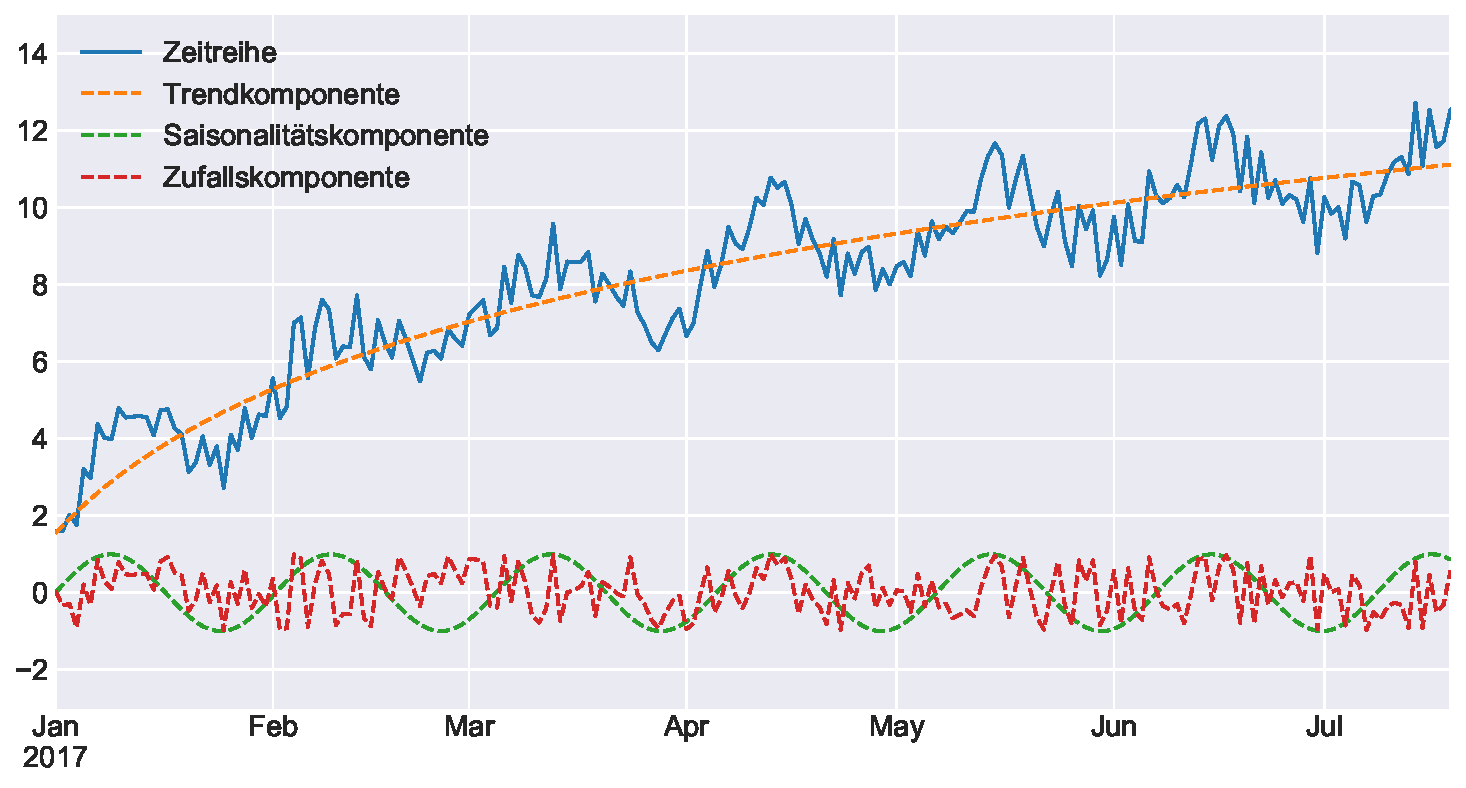
\includegraphics[width=\textwidth]{bilder/02-hauptteil/zeitreihe-komponenten.pdf}
  \caption[Aufteilung einer Zeitreihe in mehrere Komponenten]{Aufteilung einer Zeitreihe in mehrere Komponenten. Bild entnommen aus \citet{Masterthesis.2017}.}
  \label{fig:zeitreihe-komponenten}
\end{figure}


\section{Schriften}
\subsection{Schriftarten}

\textrm{textrm} \textsf{textsf} \texttt{texttt}
\textup{textup} \textsl{textsl} \textit{textit} \textsc{textsc}
\textmd{textmd} \textbf{textbf}

\subsubsection{textrm}
\textrm{
  \textmd{\upshape upshape \slshape slshape \itshape itshape \scshape scshape}
  \textbf{\upshape upshape \slshape slshape \itshape itshape \scshape scshape}
}

\subsubsection{textsf}
\textsf{
  \textmd{\upshape upshape \slshape slshape \itshape itshape \scshape scshape}
  \textbf{\upshape upshape \slshape slshape \itshape itshape \scshape scshape}
}

\subsubsection{texttt}
\texttt{
  \textmd{\upshape upshape \slshape slshape \itshape itshape \scshape scshape}
  \textbf{\upshape upshape \slshape slshape \itshape itshape \scshape scshape}
}

\subsection{Schriftgrößen}
{
\tiny tiny
\scriptsize scriptsize
\footnotesize footnotesize
\small small
\normalsize normalsize
\large large
\Large Large
\LARGE LARGE
\huge huge
\Huge Huge
}


\section{Algorithmen}
\label{sec:algorithmen}

Algorithmus \ref{alg:erstroutenplanung} zeigt auf, wie eine Generierung einer mäanderförmigen Erstroutenplanung erfolgt \citep[S.~42]{Bachelorthesis.2016}.

\begin{algorithm}
  \caption{Mäanderförmige Erstroutenplanung}
  \label{alg:erstroutenplanung}
  \begin{algorithmic}[1]
    \Require{
      \parbox[t]{.89\linewidth}{
        Flugzellenmatrizen $X^{m\times n}\;,Y^{m\times n}$
      }
    }
    \Ensure{Flugroute $F=(f_1,\; f_2,\; \dots,\; f_n)$}
    \Procedure{GetMeanderFlightRoute}{$X, Y$}
    \State $F=()$
    \State $a=1$

    \For{$i = 1:m$}
      \If{$i \bmod 2 \neq 0$}
        \For{$j = 1:n$}
          \State $f_a = (x_{ij}, y_{ij})$
          \State $a=a+1$
        \EndFor
      \Else
        \For{$j = n:1$}
          \State $f_a = (x_{ij}, y_{ij})$
          \State $a=a+1$
        \EndFor
      \EndIf
    \EndFor

    \State \Return $F$

    \EndProcedure
  \end{algorithmic}
\end{algorithm}


\section{Literaturverweise}
\label{sec:literaturverweise}

Ich bin ein \textbf{Paper} \citep[S. 234]{Chang2006}.\newline
Ich bin ein \textbf{Buch} \citep[S. 20f.]{Goll2014}. \newline
Ich bin eine \textbf{Buch-Section} \citep[S. 55ff.]{Bolanos2013} \newline
Ich bin ein \textbf{Inproceedings} \citep[]{Rodenberg2013} \newline
Ich bin eine \textbf{Internetquelle} \citep[]{Caserta2014}. \newline


\clearpage
\section{Listings}
\label{sec:listings}

Listing \ref{lst:punktinpolygon} ist direkt in das Latexdokument eingebettet.
\begin{code}
  \begin{lstlisting}[firstnumber=11,language=java]
public boolean enthaeltKoordinate( double lat, double lng ) {

    boolean ungAnzSchnittpkt = false;
    int i, j = polyKanten - 1;

    for( i = 0; i < polyKanten; i++ ) {
        if(( LngArr[ i ] < lng && LngArr[ j ] >= lng ) ||
           ( LngArr[ j ] < lng && LngArr[ i ] >= lng )) {
            if( LatArr[ i ] + (( lng - LngArr[ i ] ) /
              ( LngArr[ j ] - LngArr[ i ] ) * ( LatArr[ j ] - LatArr[ i ] )) >= lat ) {
                ungAnzSchnittpkt = !ungAnzSchnittpkt;
            }
        }
        j = i;
    }
    return ungAnzSchnittpkt;
} // Ende enthaeltKoordinate()-Methode
  \end{lstlisting}
  \caption[Auszug der PunktInPolygon-Klasse]{Auszug der \texttt{PunktInPolygon}-Klasse. Dieser zeigt die Implementierung des Punkt-in-Polygon Algorithmus.}
  \label{lst:punktinpolygon}
\end{code}

Listing \ref{lst:punktinpolygon2} ist direkt in das Latexdokument eingebettet und in der Schriftart \texttt{\textbackslash sffamily}.
\begin{code}
  \begin{lstlisting}[firstnumber=11,language=java,basicstyle={\footnotesize\sffamily}]
public boolean enthaeltKoordinate( double lat, double lng ) {

    boolean ungAnzSchnittpkt = false;
    int i, j = polyKanten - 1;

    for( i = 0; i < polyKanten; i++ ) {
        if(( LngArr[ i ] < lng && LngArr[ j ] >= lng ) ||
           ( LngArr[ j ] < lng && LngArr[ i ] >= lng )) {
            if( LatArr[ i ] + (( lng - LngArr[ i ] ) /
              ( LngArr[ j ] - LngArr[ i ] ) * ( LatArr[ j ] - LatArr[ i ] )) >= lat ) {
                ungAnzSchnittpkt = !ungAnzSchnittpkt;
            }
        }
        j = i;
    }
    return ungAnzSchnittpkt;
} // Ende enthaeltKoordinate()-Methode
  \end{lstlisting}
  \caption[Auszug der PunktInPolygon-Klasse]{Auszug der \texttt{PunktInPolygon}-Klasse. Dieser zeigt die Implementierung des Punkt-in-Polygon Algorithmus.}
  \label{lst:punktinpolygon2}
\end{code}


Der Quelltext aus Listing \ref{lst:collector-chillii} wird aus einer Datei geladen. Es wurde eine Funktion in die Einstellungen eingebaut, mit der das teilweise Anzeigen einer Quelltextdatei leicht möglich ist. Der Befehl lautet\\
\texttt{\scriptsize |\textbackslash nextline[Tabeinrückung]\{Zeilennummer der nächsten Zeile\}\{Kommentar für die ausgelassenen Zeilen\}|}.\\
Beispiel sind
\begin{enumerate} \footnotesize
  \item \texttt{|\textbackslash nextline\{24\}|}
  \item \texttt{|\textbackslash nextline[4]\{24\}|}
  \item \texttt{|\textbackslash nextline\{24\}\{Exception Handling\}|}
  \item \texttt{|\textbackslash nextline[4]\{24\}\{Exception Handling\}|}
\end{enumerate}




\begin{code}
  \lstinputlisting[language=Python]{sourcecode/collector.py}
  \caption[Collector-Skript für den System Controller]{Auszug aus dem Collector-Skript \texttt{chillii-collector/collector.py} für das Auslesen von Sensorwerten des System Controllers über die Modbus-Schnittstelle. Auszüge entnommen von \url{https://github.com/smueller18/chillii-collector/blob/1.0/collector.py}.}
  \label{lst:collector-chillii}
\end{code}


\section{Abkürzungen}
\label{sec:Abkürzungen}

\subsection{\acrlongpl{bps}}

\gu Das menschliche Gehirn nimmt ab etwa 14 bis 16 \acrlongpldat{bps} (individuell verschieden) aufeinanderfolgende Bilder als bewegte (aber nicht unbedingt ruckelfreie) Szene wahr, weswegen die Bildfrequenz in der Anfangszeit der bewegten Bilder (Stummfilmzeit), nach einer experimentellen Phase, auf 16 \acrlong{bps} festgelegt wurde. Auf dem zweiten internationalen Kongress der Filmhersteller von Paris 1909 wurden 1000 Bilder in der Minute festgelegt, was in etwa 16–17 \acrlongpl{bps} entspricht. Viele späte Stummfilme wurden jedoch mit höheren Bildfrequenzen, wie z. B. 22 \acrlongpldat{bps}, aufgenommen. Mit der Einführung des Tonfilms wurde die Bildfrequenz auf 24 Hz festgelegt.\go \citep{www:wikipedia:bildfrequenz.2017}.

\section{Formeln}

Seien $a$ und $b$ die Katheten und $c$ die Hypothenuse, dann gilt $c^{2} = a^{2} + b^{2}$ (Pythagoreischer Lehrsatz).

Seien $a$ und $b$ die Katheten und $c$ die Hypothenuse, dann gilt
  \[ c^{2} = a^{2} + b^{2} \]
(Pythagoreischer Lehrsatz).

Seien $a$ und $b$ die Katheten und $c$ die Hypothenuse, dann gilt
  \begin{equation}\label{eq:pyth2}
    c^{2} = a^{2} + b^{2}
  \end{equation}
(Pythagoreischer Lehrsatz).

\begin{eqnarray}
  f(x) & = & \cos x \nonumber\\
  f'(x) & = & -\sin x \nonumber\\
  \int_{0}^{x} f(t) dt & = & \sin(x)
\end{eqnarray}

Summenzeichen mit Indizes rechts ($\sum_{i=1}^{\infty} \frac{x^n}{n!}$) und unten bzw. oben ($\sum\limits_{i=1}^{\infty} \frac{x^n}{n!}$).

\ref{eq:matrix-x} zeigt eine Definition einer Matrix.
\begin{equation} \label{eq:matrix-x}
  X =
  \begin{pmatrix}
    x_{11} & x_{12} & \cdots  & x_{1n} \\
    x_{21} & x_{22}  & \cdots & x_{2n} \\
    \vdots  & \vdots & \ddots & \vdots \\
    x_{m1} & x_{m2} & \hdots  & x_{mn}
  \end{pmatrix}
  , x_{ij} \in \mathbb{R}
\end{equation}

\begin{equation}
f(x) =
  \left\{
    \begin{array}{l@{\quad}l}
      0, &  x\leq 0\\
      x^2 & x>0
    \end{array}
  \right.
\end{equation}

\section{Tabellen}
\label{sec:tabellen}

Anstatt \texttt{multicolumn} kann auch einfach nur \texttt{mc} benutzt werden.


\ref{tbl:eigenschaftsuebersicht-der-drohne} zeigt die Systemparameter eines Flugroboters der sitebots GmbH.
\begin{table}[h]
  \centering
  \begin{threeparttable}
    \makebox[\linewidth]{%
      \renewcommand{\TPTminimum}{\linewidth}
      \begin{tabular}{crr@{ }l}
        \toprule

        Eigenschaft & \mc{3}{c}{Wert} \\

        \cmidrule[0.4pt](r{0.25em}){1-1} \cmidrule[0.4pt](lr{0.25em}){2-4}

        Gewicht (ohne Beladung) & $=$ & 4 & \SI{}{\kilogram} \\
        Gewicht (mit Beladung) & $=$ & 5,2 & \SI{}{\kilogram} \\
        durchschnittliche Flugdauer\tnote{1)} & $\approx$ & 20 & \SI{}{\minute} \\
        Durchmesser & $=$ & 1 & \SI{}{\meter} \\
        Fluggeschwindigkeit\tnote{2)} & $\leq$ & 20 & \SI{}{\meter\per\second} \\
        Flughöhe\tnote{3)} & $\leq$ & 100 & \SI{}{\meter} \\

        \bottomrule
      \end{tabular}
    }
    \begin{tablenotes}
      \footnotesize
      \item[1)] Entspricht der durchschnittlichen Flugdauer pro Akkuladung und kann durch Wechseln von Akkus beliebig erweitert werden.
      \item[2)] Bei einer Geschwindigkeit von \SI{20}{\meter\per\second} beträgt der Anstellwinkel \SI{20}{\degree} über der Horizontalen.
      \item[3)] In der Praxis auf \SI{100}{\meter} begrenzt durch die allgemeine Aufstiegserlaubnis über Grund.
    \end{tablenotes}
  \end{threeparttable}
  \caption[Systemparameter der Drohne]{Systemparameter der Drohne nach \citet[S.~9]{Bachelorthesis.2016}}
  \label{tbl:eigenschaftsuebersicht-der-drohne}
\end{table}


\begin{table}[ht]
  \centering
  % Tabular example from LaTeX manual, p.205
  \begin{tabular}{|r||r@{--}l|p{38mm}|}
    \hline
    \mc{4}{|c|}{GG\&A Hoofed Stock}\\ \hline \hline
     & \mc{2}{c|}{Price} & \\ \cline{2-3}
    \mc{1}{|c||}{Year} & \mc{1}{r@{\,\vline\,}}{low} & high & \mc{1}{c|}{Comments} \\ \hline
    1971 & 97 & 245 & Bad year for farmers in the west. \\ \hline
      72 & 245 & 245 & Light trading due to a heavy winter. \\ \hline
      73 & 245 & 2001 & No gnus was very good gnus this year. \\ \hline
  \end{tabular}
  \caption[GG\&A Hoofed Stock]{GG\&A Hoofed Stock. Tabelle mit Priotität der Position unmittelbar an der Stelle im Quellcode durch kennzeichnen mit \texttt{ht}. Abgeändert übernommen von \url{https://mirror.hmc.edu/ctan//info/examples/lb2/5-7-8.ltx}.}
\end{table}

\section{Bilder}

\ref{fig:zeitreihe-komponenten} wurde mit dem Python Skript \verb|skripte/plot_zeitreihe_komponenten.py| erstellt.

\begin{figure}[h]
  \centering
  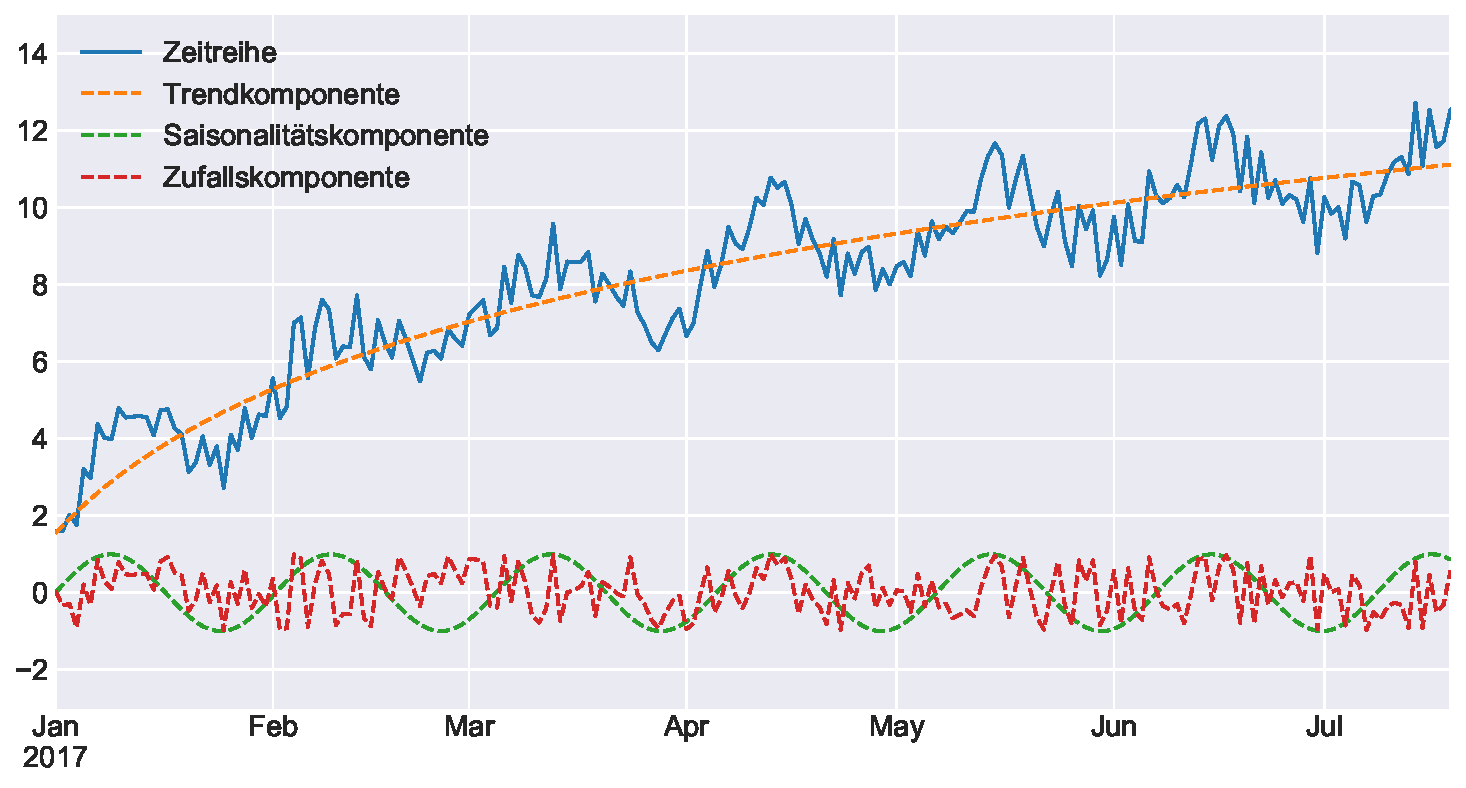
\includegraphics[width=\textwidth]{bilder/02-hauptteil/zeitreihe-komponenten.pdf}
  \caption[Aufteilung einer Zeitreihe in mehrere Komponenten]{Aufteilung einer Zeitreihe in mehrere Komponenten. Bild entnommen aus \citet{Masterthesis.2017}.}
  \label{fig:zeitreihe-komponenten}
\end{figure}

\section{Schriften}
\subsection{Schriftarten}

\textrm{textrm} \textsf{textsf} \texttt{texttt}
\textup{textup} \textsl{textsl} \textit{textit} \textsc{textsc}
\textmd{textmd} \textbf{textbf}

\subsubsection{textrm}
\textrm{
  \textmd{\upshape upshape \slshape slshape \itshape itshape \scshape scshape}
  \textbf{\upshape upshape \slshape slshape \itshape itshape \scshape scshape}
}

\subsubsection{textsf}
\textsf{
  \textmd{\upshape upshape \slshape slshape \itshape itshape \scshape scshape}
  \textbf{\upshape upshape \slshape slshape \itshape itshape \scshape scshape}
}

\subsubsection{texttt}
\texttt{
  \textmd{\upshape upshape \slshape slshape \itshape itshape \scshape scshape}
  \textbf{\upshape upshape \slshape slshape \itshape itshape \scshape scshape}
}

\subsection{Schriftgrößen}
{
\tiny tiny
\scriptsize scriptsize
\footnotesize footnotesize
\small small
\normalsize normalsize
\large large
\Large Large
\LARGE LARGE
\huge huge
\Huge Huge
}

\section{Algorithmen}
\label{sec:algorithmen}

Algorithmus \ref{alg:erstroutenplanung} zeigt auf, wie eine Generierung einer mäanderförmigen Erstroutenplanung erfolgt \citep[S.~42]{Bachelorthesis.2016}.

\begin{algorithm}
  \caption{Mäanderförmige Erstroutenplanung}
  \label{alg:erstroutenplanung}
  \begin{algorithmic}[1]
    \Require{
      \parbox[t]{.89\linewidth}{
        Flugzellenmatrizen $X^{m\times n}\;,Y^{m\times n}$
      }
    }
    \Ensure{Flugroute $F=(f_1,\; f_2,\; \dots,\; f_n)$}
    \Procedure{GetMeanderFlightRoute}{$X, Y$}
    \State $F=()$
    \State $a=1$

    \For{$i = 1:m$}
      \If{$i \bmod 2 \neq 0$}
        \For{$j = 1:n$}
          \State $f_a = (x_{ij}, y_{ij})$
          \State $a=a+1$
        \EndFor
      \Else
        \For{$j = n:1$}
          \State $f_a = (x_{ij}, y_{ij})$
          \State $a=a+1$
        \EndFor
      \EndIf
    \EndFor

    \State \Return $F$

    \EndProcedure
  \end{algorithmic}
\end{algorithm}

\section{Literaturverweise}
\label{sec:literaturverweise}

Ich bin ein \textbf{Paper} \citep[S. 234]{Chang2006}.\newline
Ich bin ein \textbf{Buch} \citep[S. 20f.]{Goll2014}. \newline
Ich bin eine \textbf{Buch-Section} \citep[S. 55ff.]{Bolanos2013} \newline
Ich bin ein \textbf{Inproceedings} \citep[]{Rodenberg2013} \newline
Ich bin eine \textbf{Internetquelle} \citep[]{Caserta2014}. \newline

\clearpage
\section{Listings}
\label{sec:listings}

Listing \ref{lst:punktinpolygon} ist direkt in das Latexdokument eingebettet.
\begin{code}
  \begin{lstlisting}[firstnumber=11,language=java]
public boolean enthaeltKoordinate( double lat, double lng ) {

    boolean ungAnzSchnittpkt = false;
    int i, j = polyKanten - 1;

    for( i = 0; i < polyKanten; i++ ) {
        if(( LngArr[ i ] < lng && LngArr[ j ] >= lng ) ||
           ( LngArr[ j ] < lng && LngArr[ i ] >= lng )) {
            if( LatArr[ i ] + (( lng - LngArr[ i ] ) /
              ( LngArr[ j ] - LngArr[ i ] ) * ( LatArr[ j ] - LatArr[ i ] )) >= lat ) {
                ungAnzSchnittpkt = !ungAnzSchnittpkt;
            }
        }
        j = i;
    }
    return ungAnzSchnittpkt;
} // Ende enthaeltKoordinate()-Methode
  \end{lstlisting}
  \caption[Auszug der PunktInPolygon-Klasse]{Auszug der \texttt{PunktInPolygon}-Klasse. Dieser zeigt die Implementierung des Punkt-in-Polygon Algorithmus.}
  \label{lst:punktinpolygon}
\end{code}

Listing \ref{lst:punktinpolygon2} ist direkt in das Latexdokument eingebettet und in der Schriftart \texttt{\textbackslash sffamily}.
\begin{code}
  \begin{lstlisting}[firstnumber=11,language=java,basicstyle={\footnotesize\sffamily}]
public boolean enthaeltKoordinate( double lat, double lng ) {

    boolean ungAnzSchnittpkt = false;
    int i, j = polyKanten - 1;

    for( i = 0; i < polyKanten; i++ ) {
        if(( LngArr[ i ] < lng && LngArr[ j ] >= lng ) ||
           ( LngArr[ j ] < lng && LngArr[ i ] >= lng )) {
            if( LatArr[ i ] + (( lng - LngArr[ i ] ) /
              ( LngArr[ j ] - LngArr[ i ] ) * ( LatArr[ j ] - LatArr[ i ] )) >= lat ) {
                ungAnzSchnittpkt = !ungAnzSchnittpkt;
            }
        }
        j = i;
    }
    return ungAnzSchnittpkt;
} // Ende enthaeltKoordinate()-Methode
  \end{lstlisting}
  \caption[Auszug der PunktInPolygon-Klasse]{Auszug der \texttt{PunktInPolygon}-Klasse. Dieser zeigt die Implementierung des Punkt-in-Polygon Algorithmus.}
  \label{lst:punktinpolygon2}
\end{code}


Der Quelltext aus Listing \ref{lst:collector-chillii} wird aus einer Datei geladen. Es wurde eine Funktion in die Einstellungen eingebaut, mit der das teilweise Anzeigen einer Quelltextdatei leicht möglich ist. Der Befehl lautet\\
\texttt{\scriptsize |\textbackslash nextline[Tabeinrückung]\{Zeilennummer der nächsten Zeile\}\{Kommentar für die ausgelassenen Zeilen\}|}.\\
Beispiel sind
\begin{enumerate} \footnotesize
  \item \texttt{|\textbackslash nextline\{24\}|}
  \item \texttt{|\textbackslash nextline[4]\{24\}|}
  \item \texttt{|\textbackslash nextline\{24\}\{Exception Handling\}|}
  \item \texttt{|\textbackslash nextline[4]\{24\}\{Exception Handling\}|}
\end{enumerate}




\begin{code}
  \lstinputlisting[language=Python]{sourcecode/collector.py}
  \caption[Collector-Skript für den System Controller]{Auszug aus dem Collector-Skript \texttt{chillii-collector/collector.py} für das Auslesen von Sensorwerten des System Controllers über die Modbus-Schnittstelle. Auszüge entnommen von \url{https://github.com/smueller18/chillii-collector/blob/1.0/collector.py}.}
  \label{lst:collector-chillii}
\end{code}



% Anhang
\appendix
\addchap{Anhang}
\label{chap:anhang}

\section{Section}

\subsection{Subsection 1}
\subsubsection{Subsubsection 1}
\subsubsection{Subsubsection 2}

\subsection{Subsection 2}
\subsubsection{Subsubsection 1}
\subsubsection{Subsubsection 2}

\section{Quelltexte}
\label{sec:quelltexte}


\begin{code}
  \lstinputlisting[language=tex]{sourcecode/LICENSE}
  \caption{MIT Lizenz}
  \label{lst:mitlizenz}
\end{code}


\section{Algorithmen}

Algorithmus \ref{alg:erstroutenplanung-anhang} zeigt auf, wie eine Generierung einer mäanderförmigen Erstroutenplanung erfolgt \citep[S.~42]{Bachelorthesis.2016}.

\begin{algorithm}
  \caption{Mäanderförmige Erstroutenplanung}
  \label{alg:erstroutenplanung-anhang}
  \begin{algorithmic}[1]
    \Require{
      \parbox[t]{.89\linewidth}{
        Flugzellenmatrizen $X^{m\times n}\;,Y^{m\times n}$
      }
    }
    \Ensure{Flugroute $F=(f_1,\; f_2,\; \dots,\; f_n)$}
    \Procedure{GetMeanderFlightRoute}{$X, Y$}
    \State $F=()$
    \State $a=1$

    \For{$i = 1:m$}
      \If{$i \bmod 2 \neq 0$}
        \For{$j = 1:n$}
          \State $f_a = (x_{ij}, y_{ij})$
          \State $a=a+1$
        \EndFor
      \Else
        \For{$j = n:1$}
          \State $f_a = (x_{ij}, y_{ij})$
          \State $a=a+1$
        \EndFor
      \EndIf
    \EndFor

    \State \Return $F$

    \EndProcedure
  \end{algorithmic}
\end{algorithm}

\section{Bilder}

Bilder aus dem Anhang werden nicht im Abbildungsverzeichnis aufgeführt, daher ist dort auch kein Link zu \ref{fig:zeitreihe-komponenten4}.

\begin{figure}[h]
  \centering
  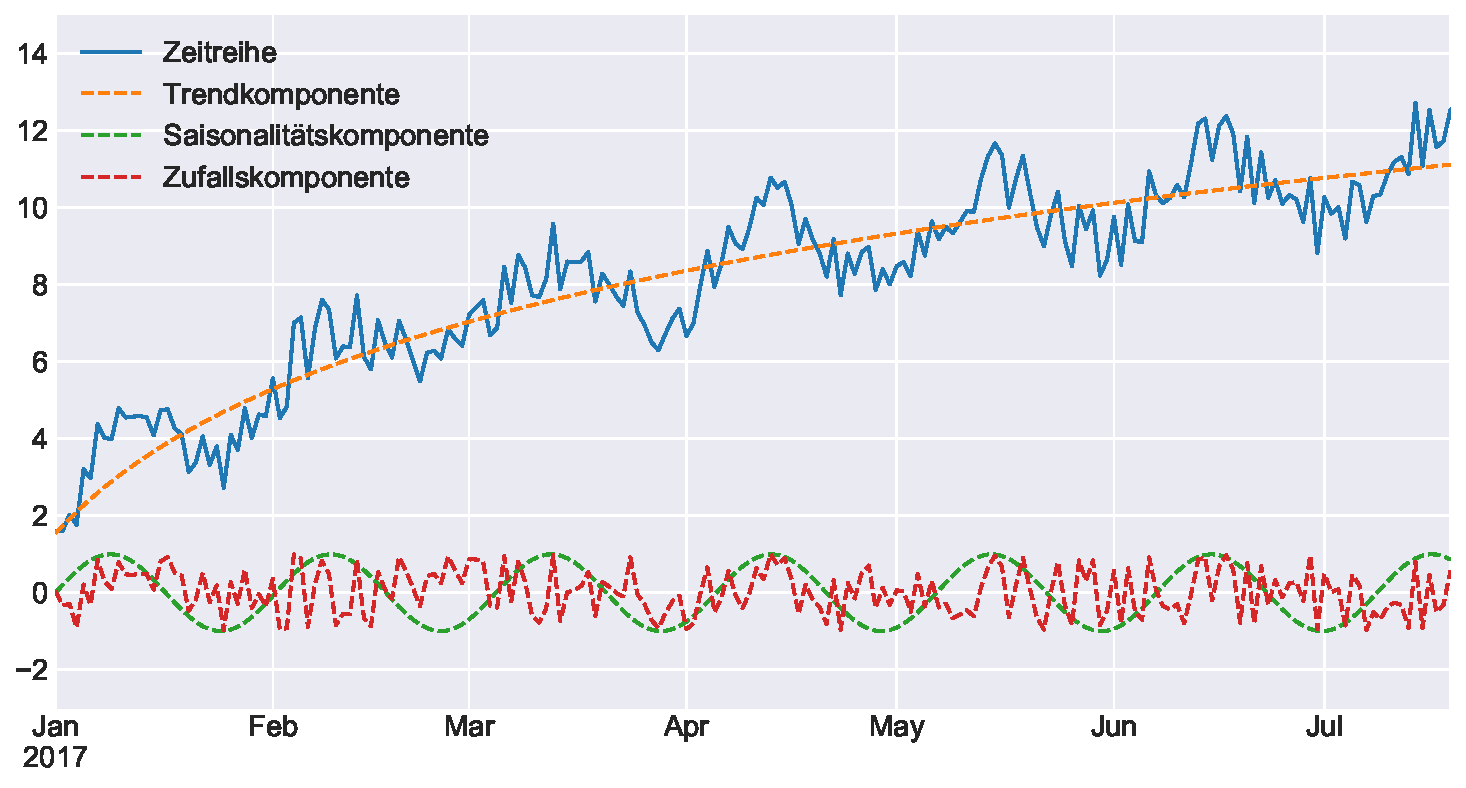
\includegraphics[width=\textwidth]{bilder/02-hauptteil/zeitreihe-komponenten.pdf}
  \caption[Aufteilung einer Zeitreihe in mehrere Komponenten]{Aufteilung einer Zeitreihe in mehrere Komponenten. Bild entnommen aus \citet{Masterthesis.2017}.}
  \label{fig:zeitreihe-komponenten4}
\end{figure}

\section{Tabelle}
\ref{tbl:gg-hoofed-stock} ist eine Tabelle im Anhang.
\begin{table}[ht]
  \centering
  % Tabular example from LaTeX manual, p.205
  \begin{tabular}{|r||r@{--}l|p{38mm}|}
    \hline
    \mc{4}{|c|}{GG\&A Hoofed Stock}\\ \hline \hline
     & \mc{2}{c|}{Price} & \\ \cline{2-3}
    \mc{1}{|c||}{Year} & \mc{1}{r@{\,\vline\,}}{low} & high & \mc{1}{c|}{Comments} \\ \hline
    1971 & 97 & 245 & Bad year for farmers in the west. \\ \hline
      72 & 245 & 245 & Light trading due to a heavy winter. \\ \hline
      73 & 245 & 2001 & No gnus was very good gnus this year. \\ \hline
  \end{tabular}
  \caption[GG\&A Hoofed Stock]{GG\&A Hoofed Stock. Tabelle mit Priotität der Position unmittelbar an der Stelle im Quellcode durch kennzeichnen mit \texttt{ht}. Abgeändert übernommen von \url{https://mirror.hmc.edu/ctan//info/examples/lb2/5-7-8.ltx}.}
  \label{tbl:gg-hoofed-stock}
\end{table}


\section{Inhalte des beiliegenden Datenträgers}
\label{sec:quelltexte}

\begin{figure}[H]
  \begin{minipage}[T]{\textwidth}
    \dirtree{%
      .1 Datenträger.
        .2 Thesis/ \ldots\DTcomment{ Masterthesis als Latex-Dokument}.
        .2 Onlinequellen/ \ldots\DTcomment{ Verwendete Onlinequellen als \texttt{pdf}-Datei}.
        .2 Quelltexte/ \ldots\DTcomment{ Klon aller erstellten Git-Projekte}.
          .3 chillii-collector\footnote{\url{https://github.com/smueller18/chillii-collector}}.
        .2 thesis.pdf \ldots\DTcomment{ Thesis als \texttt{pdf}-Datei}.
    }
  \end{minipage}

  \caption{Verzeichnisstruktur der beiliegenden CD}
  \label{fig:cd}
\end{figure}


% Literaturverzeichnis
\bibliographystyle{natdin}
\bibliography{literatur}
\clearpage

% Springe an richtige Position beim Anklicken des Inhaltsverzeichniseintrags
\phantomsection
\addcontentsline{toc}{chapter}{Eidesstattliche Erklärung}

\chapter*{Eidesstattliche Erklärung}
\thispagestyle{empty}

Hiermit erkläre ich, dass ich die vorliegende Arbeit selbstständig und nur unter Benutzung der angegebenen Quellen und Hilfsmittel angefertigt habe. Alle Textstellen, die wörtlich oder sinngemäß aus veröffentlichten oder nicht veröffentlichten Quellen entnommen wurden, sind als solche kenntlich gemacht. Die Arbeit hat in gleicher oder ähnlicher Form keiner anderen Prüfungsbehörde vorgelegen.
\vspace{2\baselineskip}

\noindent Karlsruhe, den 1. Januar \the\year
\begin{flushright}
	\parbox{5cm}{
		\rule{5cm}{.5pt}
		\centering \raisebox{1.5mm}{Vorname Nachname}
	}
\end{flushright}


\end{document}
